

\section{Modeling Path Planning as a MILP problem}
\subsection{Introduction}
This section covers how a path planning problem can be represented as a mixed integer linear program. As mentioned before, the way the problem is represented is based on the work by Schouwenaars et al. \cite{Schouwenaars2001}.
\subsection{Overview of MILP}
\label{subsec:previous}
Mixed integer linear programming is and extension of linear programming. In a linear programming problem, there is a single (linear) target function which needs to be minimized or maximized by the solver. A problem typically also contains a number linear inequalities which constrain the values of the variables in the target function. \\
\begin{figure}
\begin{math}
\text{maximize} \quad f(\boldsymbol{x}) = a_0 x_0 + a_1 x_1 + ...\\
\text{subject to} \\
b_{0,0} x_0 + b_{0,1} x_1 + ...\leq c_0 \\
b_{1,0} x_0 + b_{1,1} x_1 + ...\leq c_1 \\
... \\
x_0, x_1, ... \in \mathbb{R}
\end{math}
\caption{A typical linear problem}
\label{fig:example-lp}
\end{figure}
In the example in figure \ref{fig:example-lp}, $  f(\boldsymbol{x}) $ is the linear goal function to be maximized. When a symbol is in \textbf{bold}, it represents a vector, otherwise it represents a scalar value. In this case, $\boldsymbol{x}$ is the vector containing all variables $x_i$. The linear inequalities below the goal function are the constraints as linear inequalities with coefficients $b_{j,i}$ and the maximum value $c_j$. The final line ensures that all variables have a real domain. When some (or all) of the variables have an integer domain, the program is called mixed integer. \\
Using multiple inequalities and possibly additional variables, it is possible to model more complex mathematical relations. Some of those relations, like logical operators, can only be expressed when integer variables are allowed \cite{Mitra1994}. 
\subsection{Time and vehicle state}
\label{section:modeling}

The path planning problem can be represented with discrete timesteps with a set of state variables for each epoch. The amount of timesteps determines the maximum amount of time the vehicle has in solution space to reach its goal. The actual movement of the vehicle is modeled by calculating the accelleration, velocity and position at each timestep based on the throttle (in each axis) and state variables from the previous time step.

\begin{equation}
\label{eq:t-start}
time_0 = 0
\end{equation}
\begin{equation}
\label{eq:t-rest}
time_{t+1} = time_{t} + \Delta t,  \quad 0 \leq t < N
\end{equation}

Equation \ref{eq:t-start} and \ref{eq:t-rest} model the progress of time. $time_t$ represents the current time at timestep $t$. $\Delta t$ is the duration of a single time step. There are $N + 1$ timesteps.


\begin{equation}
\label{eq:p-start}
\boldsymbol{p}_0 = \boldsymbol{p}_{start}
\end{equation}
\begin{equation}
\label{eq:p-rest}
\boldsymbol{p}_{t+1} = \boldsymbol{p}_{t} + \Delta t * \boldsymbol{v}_{t}  \quad 0 \leq t < N
\end{equation}

Equation \ref{eq:p-start} and \ref{eq:p-rest} model the position of the vehicle at each time step. $p_0$ is initialized with a certain starting position $p_{start}$. For each time step $t$, the position in the next time step $p_{t+1}$ is determined by the current position $p_t$, the current velocity $v_t$ and the duration of the time step $\Delta t$. Note that both the position and velocity use vector notation.

\begin{equation}
\label{eq:v-start}
\boldsymbol{v}_0 =\boldsymbol{v}_{start}
\end{equation}
\begin{equation}
\label{eq:v-rest}
\boldsymbol{v}_{t+1} =\boldsymbol{v}_{t} + \Delta t * \boldsymbol{a}_{t}  \quad 0 \leq t < N
\end{equation}

Similarly to the position, \ref{eq:v-start} and \ref{eq:v-rest} model the velocity of the vehicle at each time step. This time the starting velocity is initialized with $v_{start}$ and updated based on the current velocity and current acceleration.\\
The acceleration can be modeled the same way based on the jerk, which can in turn be modeled based on the snap, etc. How many derivates need to be modeled will vary depending on the specific use case.

\subsection{Goal function}
The problem also needs a goal function to optimize. In this model, the goal is to minimize the time before a goal position is reached. this is expressed in equation \ref{eq:goal-fun}. Reaching the goal causes a state transition from not being finished to being finished. This is represented as the value of $fin_t$, which is a binary variable (which is an integer variable which can only be 0 or 1). When $fin_t$ is true, the has reached its goal on or before time step $t$.
\begin{equation}
\label{eq:goal-fun}
minimize \quad N - \mathlarger{\sum}_{t=0}^{t \leq N} fin_t
\end{equation}
\begin{equation}
\label{eq:fin-start}
fin_0 = 0
\end{equation}
\begin{equation}
\label{eq:fin-end}
fin_{N} = 1
\end{equation}
\begin{equation}
\label{eq:fin-rest}
fin_{t+1} = fin_t \vee cfin_{t+1},  \quad 0 \leq t < N
\end{equation}
Equation \ref{eq:fin-start} initialized $fin_0$ to be false, ensuring that the initial state is not finished. Equation \ref{eq:fin-end} forces the state in the last time step to be finished. This means that the vehicle must reach its goal eventually for the problem to be considered solved. \\
Modeling state transitions directly can be error-prone, so Lamport's\cite{Lamport1989} state transition axiom method was used. In this simple model it is still possible to model the state transition directly, but this notation is much easier to extend. In equation \ref{eq:fin-rest}, the state will be finished during timestep $t+1$ if the state is finished during timestep$t$ or if there is a state transition from not finished to finished at timestep $t + 1$, represented by $cfin_{t+1}$ .

\begin{equation}
\label{eq:cfin}
cfin_t =  cfin_{p,t} \wedge \neg fin_t\quad 0 \leq t \leq N
\end{equation}

 $cfin_t$ in equation \ref{eq:cfin} is true at timestep $t$ if the goal position requirement $cfin_{p,t}$ is true and the finished state has not already been reached ( $ \neg fin_t$ ). This shows the advantages of the state transition axiom method: Constraints on the state transition can easily be added and removed without having to write complex logical furmulas.
\begin{equation}
\label{eq:cfin-p}
cfin_{p,t} =  \mathlarger{\mathlarger{\bigwedge_{i = 0}^{i < Dim(\boldsymbol{p}_t)}}} |p_{t,i} - p_{goal, i}| < \epsilon_{p},  \quad 0 \leq t \leq N
\end{equation}
The goal position requirement is represented by $cfin_{p,t}$ and is satisfied when $cfin_{p,t} = 1$. The coordinate in dimension $i$ of the position vector $\boldsymbol{p}_t$, is $p_{t,i}$. The goal position coordinate in that dimension is $p_{goal, i}$. If the difference between those values is smaller than some value $\epsilon_p$ in every dimension at time step $t$,  $cfin_{p,t} = 1$.

\subsection{Vehicle state limits}

Vehicles have a maximum velocity they can achieve. Calculating the velocity of the vehicle means calculating the 2-norm of the velocity vector. This is not possible using only linear equations. However, it can be approximated to an arbitrary degree using multiple linear constraints. For simplicity we will only cover the 2D case, although this can easily be extended to 3D as well. With $x_i$ and $y_i$ the $N_{points}$ vertices of the approximating polygon listed in counter-clockwise order, the velocity can be limited to $v_{max}$ with equation \ref{eq:vmax}. Figure \ref{fig:circlelinear} shows a visual representation of this.
%\begin{equation}
%\label{eq:}
%\theta = \dfrac{2\pi}{N_{points}}
%\end{equation}
%\begin{equation}
%\label{eq:}
%x_i  = v_{max} * cos( \theta * i)
%\end{equation}
%\begin{equation}
%\label{eq:}
%y_i  = v_{max} * sin( \theta * i)
%\end{equation}
\begin{equation}
\label{eq:lin-a}
a_i = \dfrac{y_{i} - y_{i-1}}{x_{i} - x_{i-1}} \quad 0 \leq i < N_{points}
\end{equation}
\begin{equation}
\label{eq:lin-b}
b_i = y_{i} - a_i x_i  \quad 0 \leq i < N_{points}
\end{equation}
\begin{equation}
\label{eq:vmax}
v_{t, 1} \leq a_i v_{t,0} + b_i  \quad 0 \leq i < N_{points}, ~ 0 \leq t \leq N
\end{equation}

\begin{figure}
    \centering
        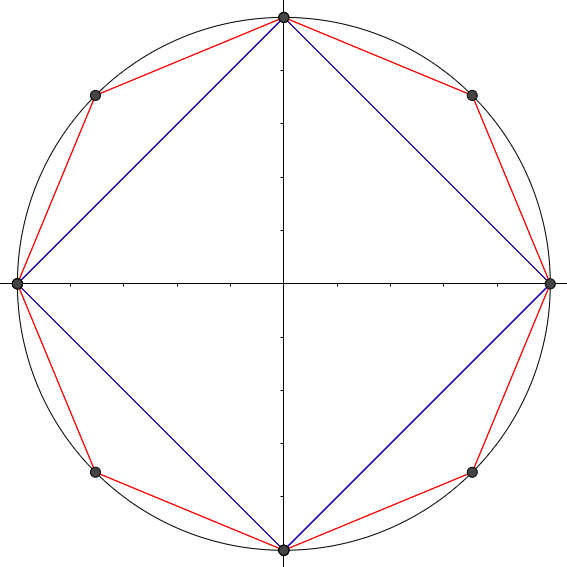
\includegraphics[width=0.7\columnwidth]{img/circlelinear}
    \caption{If the velocity is limited to a finite value, the velocity vector must lie within the circle centered on the origin with the radius equal to that value. This is represented by the black circle. This circle cannot be approximated in MILP, but it can be approximated using several linear constraints. The blue square shows the approximation using 4 linear constraints. The red polygon uses 8 linear constraints. As more constraints are used, the approximation gets closer and closer. }\label{fig:circlelinear}
\end{figure}
The acceleration and other vector properties of the vehicle can be limited in the same way. Although it is less obvious, this can also be applied to keep the vehicle's position inside a convex polygon. The importance of this will become clear section \ref{section:segment}.

\subsection{Obstacle avoidance}

\begin{figure}[!t]
    \centering
    \subfloat{
        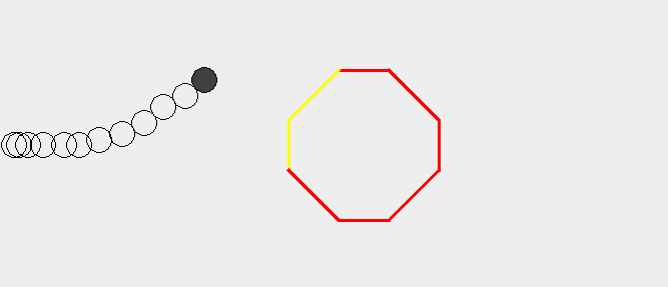
\includegraphics[width=0.9\columnwidth]{img/obs1}
    }
    \hfil
     \subfloat{
        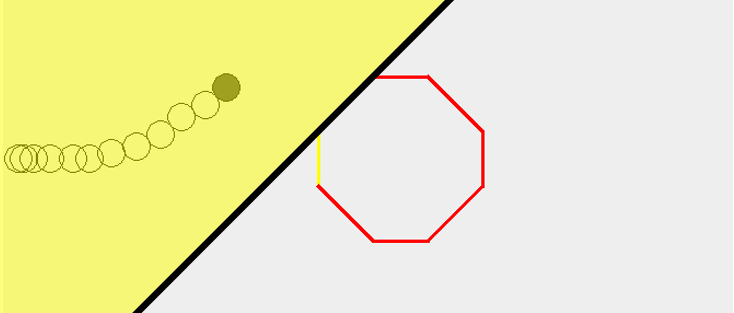
\includegraphics[width=0.9\columnwidth]{img/obs2}
     }
     \hfil
     \subfloat{
        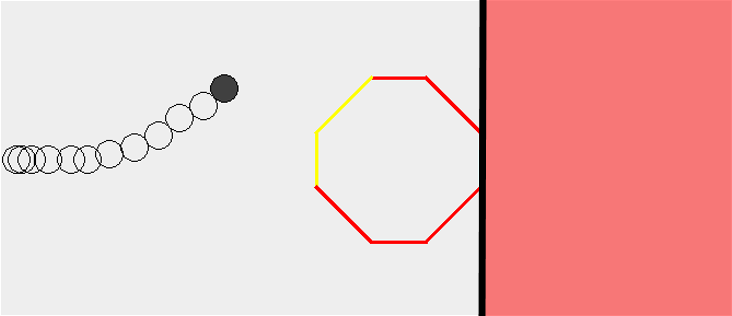
\includegraphics[width=0.9\columnwidth]{img/obs3}
     }
    \caption{A visual representation of how obstacle avoidance works. The top image shows the vehicle's current position as the filled circle, with its path in previous time steps as hollow circles. The color of the edges of the obstacle represent whether or not the vehicle is in the safe zone for that edge. An edge is yellow if the vehicle is in the safe zone, and red otherwise. The middle image shows the safe half-plane defined by a yellow edge in yellow. Note how the vehicle is on one side of the black line and the obstacle is entirely on the other side. The bottom image shows an edge for which the vehicle is not in the safe zone (represented in red this time). As long as the vehicle is in the safe zone of at least one edge, it cannot collide with the obstacle.}\label{fig:obs}
\end{figure}
The most challenging part of the problem is modeling obstacles. Any obstacle between the vehicle and its goal will inherently make the search space non-convex. Because of this, integer variables are needed to model obstacles. For each edge of the polygon obstacle, the line through that edge is constructed. If the obstacle is convex, the obstacle will be entirely on one side of that line. This means that the other side can be considered safe. However, the vehicle cannot be on the safe area of all edges at the same time, so a mechanism is needed to turn off these constraints when needed. As long as the vehicle is in the safe area of at least one edge, it cannot collide.  Figure \ref{fig:obs} demonstrates this visually. \\

The most common way to turn off individual constraints is using the ``Big M'' method, like Schouwenaars et al. \cite{Schouwenaars2001} used in their work. However CPLEX supports a better way called ``indicator constraints''. Just like with the Big M method, it requires one boolean variable per edge. If the variable is true, the corresponding constraint is ignored. As long as at least one of those variables if false, a collision cannot happen. We will call these slack variables. For every convex obstacle $o$ with vertices $x_{o,i}$ and $y_{o,i}$ with $a_{o,i}$ and $b_{o,i}$ calculated as in equations \ref{eq:lin-a} and \ref{eq:lin-b}:
\begin{equation*}
dx_{o,i} = x_{o,i} - x_{o,i-1}, \quad dy_{o,i} = y_{o,i} - y_{o,i-1}
\end{equation*}
\begin{equation}
\label{eq:obs}
slack_{o,i,t} \Rightarrow \\
\begin{cases}
b_i + buf_{o,i} \leq p_{t,1} - a_i p_{t,0} & dx_{o,i} < 0 \\
b_i - buf_{o,i}  \geq p_{t,1} - a_i p_{t,0} & dx_{o,i} > 0 \\
x_{o,i} + buf_{o,i}  \leq p_{t,0} & dx_{o,i} = 0, dy_{o,i} > 0 \\
x_{o,i} - buf_{o,i}  \geq p_{t,0} & dx_{o,i} = 0, dy_{o,i} < 0 \\
\end{cases}
\end{equation}

\begin{equation}
\neg \mathlarger{\mathlarger{\bigwedge_{i}}} slack_{o,i,t} \quad 0 \leq t \leq N
\end{equation}

The occurances of $buf_{o,i}$ in equation \ref{eq:obs} are necessary because the vehicle is not a point. With $\alpha_{o,i}$ the angle perpendicular to the edge and $S$ the radius of the vehicle:

\begin{equation}
\alpha_{o,i} = tan^{-1}( -1 / a_{o,i})
\end{equation}
\begin{equation}
buf_{o,i} = |\dfrac{S}{sin(\alpha_{o,i})}|
\end{equation}